\section{Definición de requerimientos y restricciones}

    En este capítulo se describe la metodología seguida para definir la dirección y estructura del desarrollo del aplicativo. Partiendo de una revisión de la literatura enfocada principalmente al mantenimiento preventivo y a los aspectos relacionados al manejo de la información, se planteó una encuesta que fue contestada por personas involucradas en el campo del mantenimiento, a la cual se le realizó un análisis cualitativo con el fin de concretar las secciones a incluir en la aplicación y las funcionalidades ofrecidas al usuario.

    \subsection{Análisis cualitativo}

        Se optó por un enfoque cualitativo para llevar a cabo una investigación que resultara en la obtención de características y funcionalidades a incluir en un aplicativo que asista en la gestión de  información y desarrollo de actividades de mantenimiento. Este enfoque se caracteriza por su flexibilidad y la exploración de percepciones, acciones y sentimientos de participantes mediante entrevistas, análisis de contenido, observaciones o grupos focales \parencite{BARROGA:2023}.

    \subsection{Identificación de patrones}

        Para el análisis de datos cualitativos se desarrolló una encuesta (Apéndice \ref{apc:qualitative_analysis_interview}) orientada a recopilar datos y conceptos aportados por personas con experiencia en el mantenimiento industrial, con el fin de identificar características a incluir en el aplicativo móvil de realidad aumentada y gestión de la información para el mantenimiento preventivo. La información obtenida fue sometida a un proceso sistemático de codificación, categorización y síntesis, que permitió no solo identificar patrones recurrentes sino también revelar particularidades relevantes para el desarrollo del aplicativo.

        Las entrevistas derivadas de la encuesta fueron registradas, guardadas y anonimizadas para su respectivo análisis. En ellas, se buscaba que los encuestados respondieran a partir de su experiencia en el área de mantenimiento, su familiaridad con las tecnologías de la información y la comunicación (TIC) y la realidad aumentada, así como su conocimiento sobre deficiencias organizacionales y conceptos asociados al mantenimiento preventivo.

    \subsection{Categorización y codificación}

        Se generó un conjunto de categorías a las cuales se les relacionarían posteriormente frases o citas de la transcripción de las encuestas buscando con esto clasificar y organizar la información para facilitar la identificación de patrones y vínculos conceptuales. \textcite{RODRIGUEZ:2005} mencionan que este proceso de categorización se puede realizar mediante un enfoque deductivo, en base a categorías establecidas previamente a la lectura del material; un enfoque inductivo, donde las categorías están establecidas a partir de la lectura y exámen del material; o aplicando ambos (enfoque mixto). Para el desarrollo del análisis se consideró la generación de las categorías después de realizar la lectura del texto.

        Para lograr enlazar o relacionar lo expresado en las entrevistas se enumeraron categorías, subcategorías y palabras clave, las cuales identifican una determinada frase de interés dentro del cuerpo de texto de las transcripciones, para así poder conectar las diferentes citas de los entrevistados a un tema específico, encontrando similitudes o repeticiones en algunos términos. Las categorías generadas fueron las siguientes:

        \begin{itemize}

            \item \textbf{Perfil del encuestado:} Reúne información relacionada con la experiencia en el área del mantenimiento de los encuestados, los conocimientos desarrollados a partir de esa experiencia y la familiaridad que tienen con herramientas tecnológicas en dicho contexto.

            \item \textbf{Mantenimiento preventivo:} Comprende conceptos y conocimientos asociados al mantenimiento preventivo mencionados por los entrevistados y respaldados por la literatura consultada.

            \item \textbf{Defectos organizacionales:} En esta categoría se incluyen las problemáticas asociadas al mantenimiento de equipos que los entrevistados señalaron, destacando aquellas en las que la incorporación de nuevas tecnologías, como la realidad aumentada, podría representar una mejora.

            \item \textbf{Aplicativo de realidad aumentada:} En esta categoría se hace referencia a la información asociada con los paneles y funcionalidades de un aplicativo de realidad aumentada para mantenimiento preventivo, así como los desafíos para su implementación.

        \end{itemize}

        \begin{figure}[H]
    \caption{Categorización de los códigos para análisis cualitativo}
    \centering
    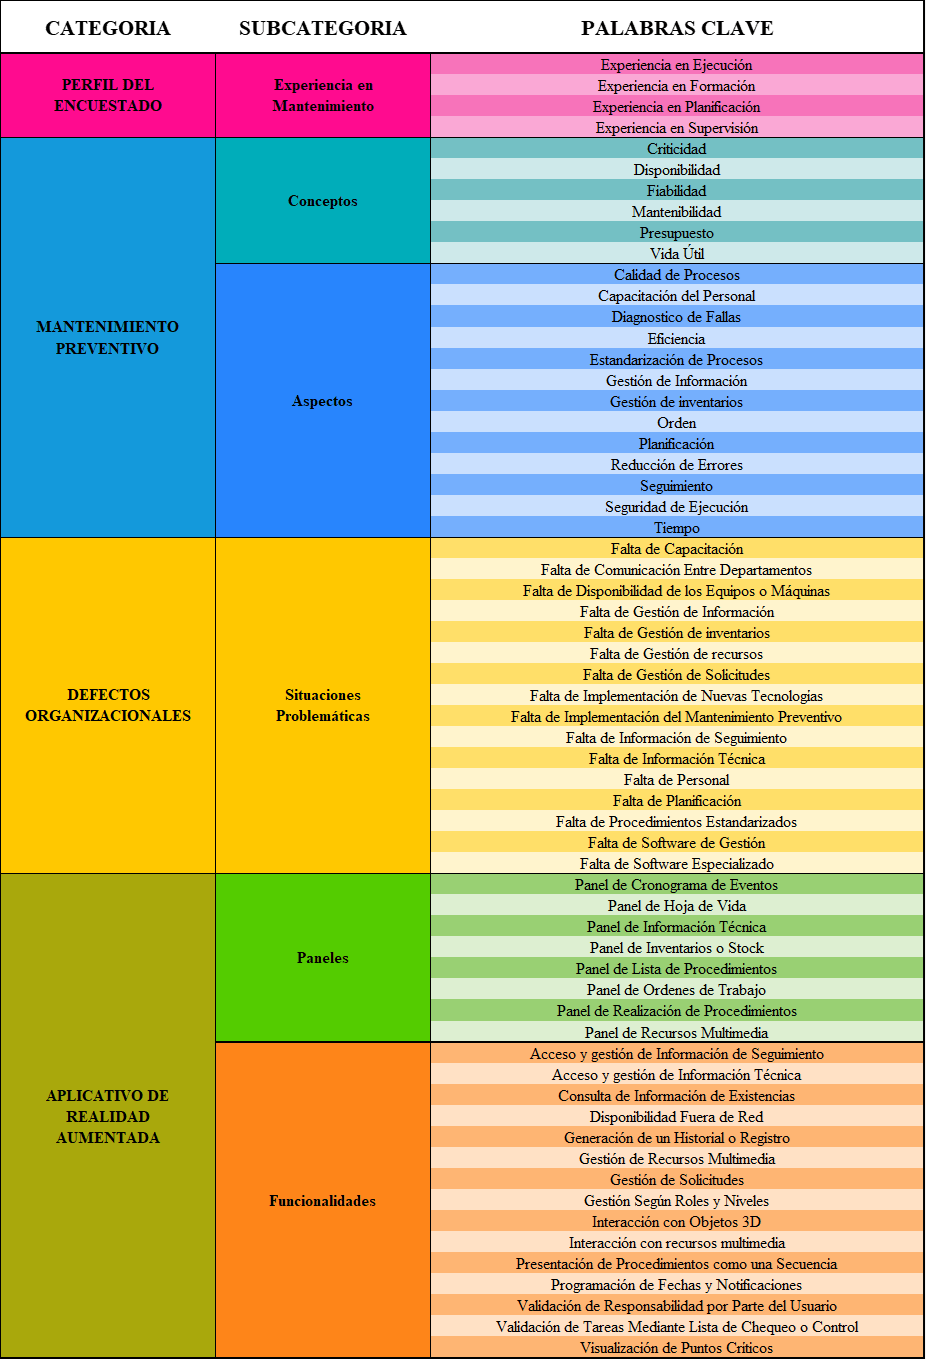
\includegraphics[width=0.9\textwidth]{assets/figures/first_phase/img_codes_categories.png}
    \label{fig:codes_categories}
\end{figure}
\fixvspace{0}

    \subsection{Uso de software de análisis cualitativo}

        Para llevar a cabo la codificación de las citas se empleó el software de análisis cualitativo ATLAS.ti. Inicialmente, se realizó una lectura exploratoria de las respuestas con el propósito de identificar segmentos de texto relevantes y asignarles códigos, tanto predefinidos en función de los objetivos del estudio como incorporados durante el proceso de análisis cuando fue necesario.

        En el análisis cualitativo es común que una misma cita sea asociada con múltiples códigos, ya que un mismo fragmento puede abordar diferentes conceptos de interés. Esta asignación simultánea da lugar a la coocurrencia de códigos, cuya exploración permite identificar patrones de asociación entre las categorías definidas durante el proceso de codificación.

        A partir de esta información, se generaron recursos gráficos, como gráficos de coocurrencia y redes de relaciones entre códigos, que facilitaron la interpretación de los vínculos existentes entre las categorías analizadas. Estos recursos contribuyen a identificar tendencias y asociaciones presentes en las respuestas de los participantes, apoyando la interpretación de los resultados obtenidos.

    \subsection{Creación de redes semánticas}

        A partir de los códigos obtenidos durante el análisis cualitativo, se generaron redes semánticas para cada uno de los paneles identificados en las encuestas. Estas estructuras presentan un patrón característico que permite vincular diversos nodos y representar cómo se interrelacionan varios conceptos \parencite{PEREZ:2022}.

        El software utilizado ofrece siete tipos de relaciones conceptuales por defecto (Figura \ref{fig:relations_default}), para facilitar la visualización de las relaciones entre diversos códigos.
        
        \begin{figure}[H]
    \caption{Relaciones por defecto de ATLAS.ti.}
    \centering
    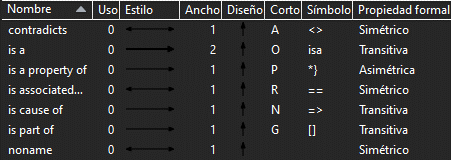
\includegraphics[width=0.6\textwidth]{assets/figures/first_phase/relation/img_relations_default.png}
    \label{fig:relations_default}
\end{figure}
\fixvspace{0}

        Sin embargo, se propusieron conectores personalizados (Figura \ref{fig:relations_proposed}) para representar con mayor precisión las relaciones entre los códigos, las funcionalidades propuestas y los aspectos del mantenimiento preventivo asociados a cada panel, con el fin de explorar su integración en el aplicativo de realidad aumentada.
        
        \begin{figure}[H]

    \caption{Conectores de relación propuestos.}
    
    \centering
    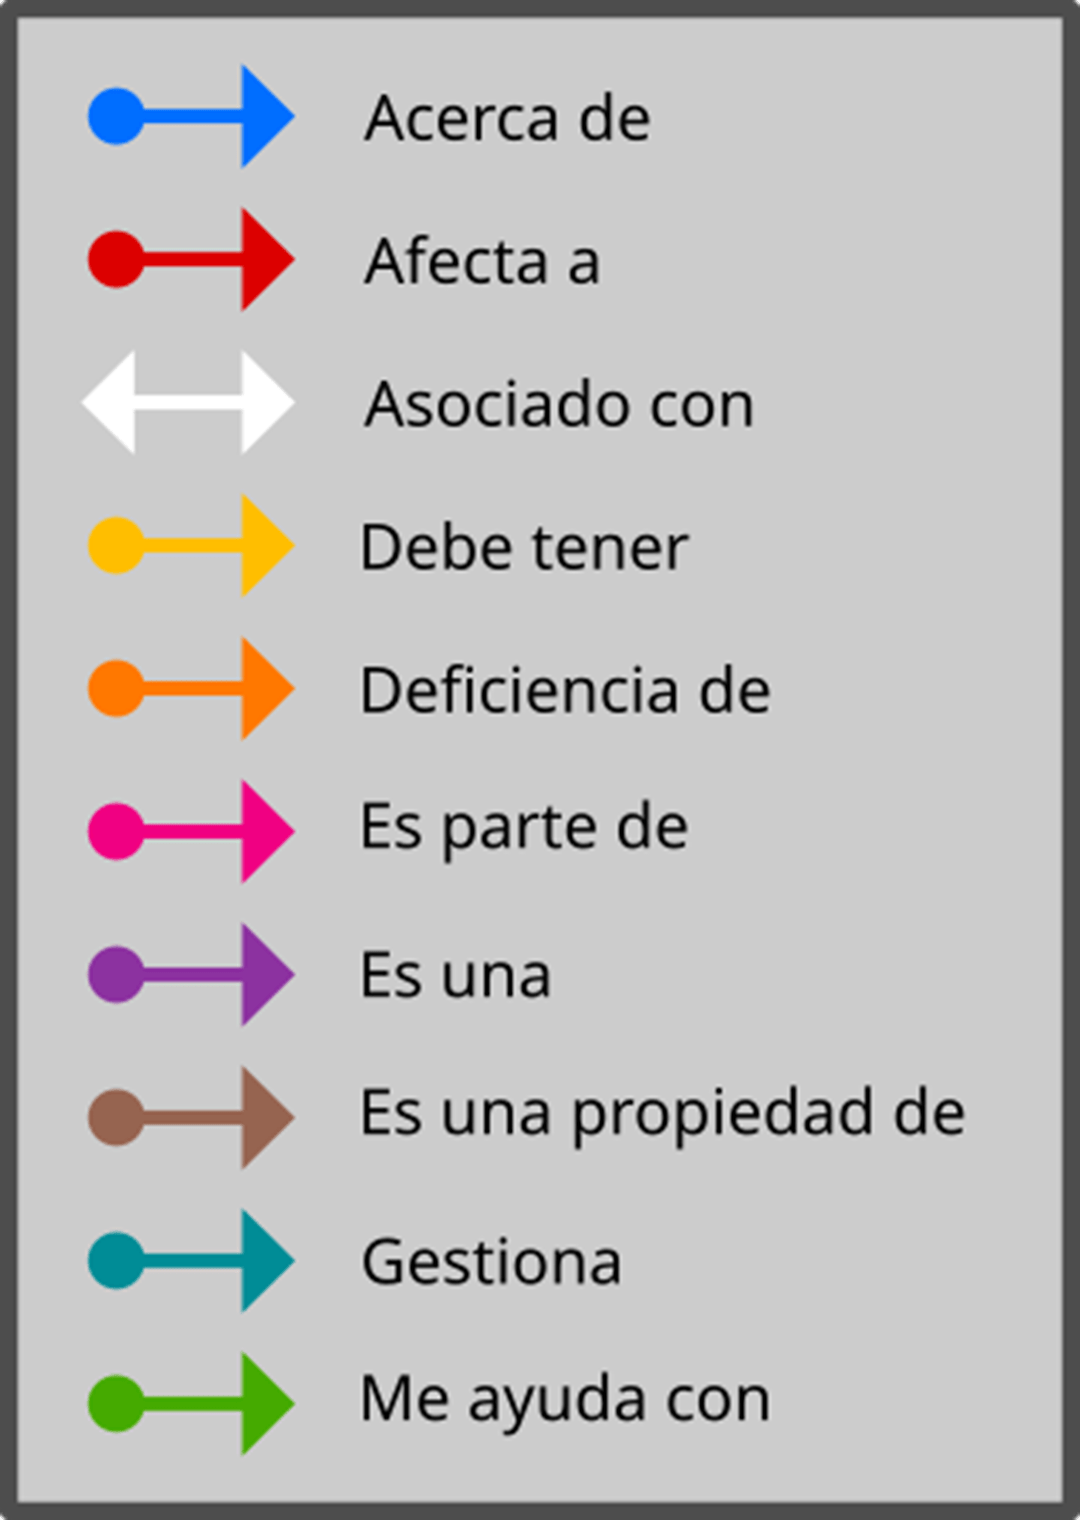
\includegraphics[width=0.3\textwidth]{assets/figures/first_phase/relation/img_relations_proposed.png}
    \label{fig:relations_proposed}
    
\end{figure}
\fixvspace{0}

        \subsubsection{Red de situaciones problemáticas}

            En la Figura \ref{fig:semantic_network_problematic_situations} Se muestra una red semántica generada a partir de la codificación de las citas, la cual refleja diversas situaciones problemáticas señaladas por los entrevistados, las cuales se identifican como causas o consecuencias de la ausencia de un determinado aspecto del mantenimiento. Esta representación evidencia la relevancia de dichos aspectos dentro de una organización, destacando cómo su omisión puede generar dificultades y afectaciones en los procesos de gestión y operación.

            \begin{figure}[H]
    \caption{Relaciones semánticas de las situaciones problemáticas}
    \centering
    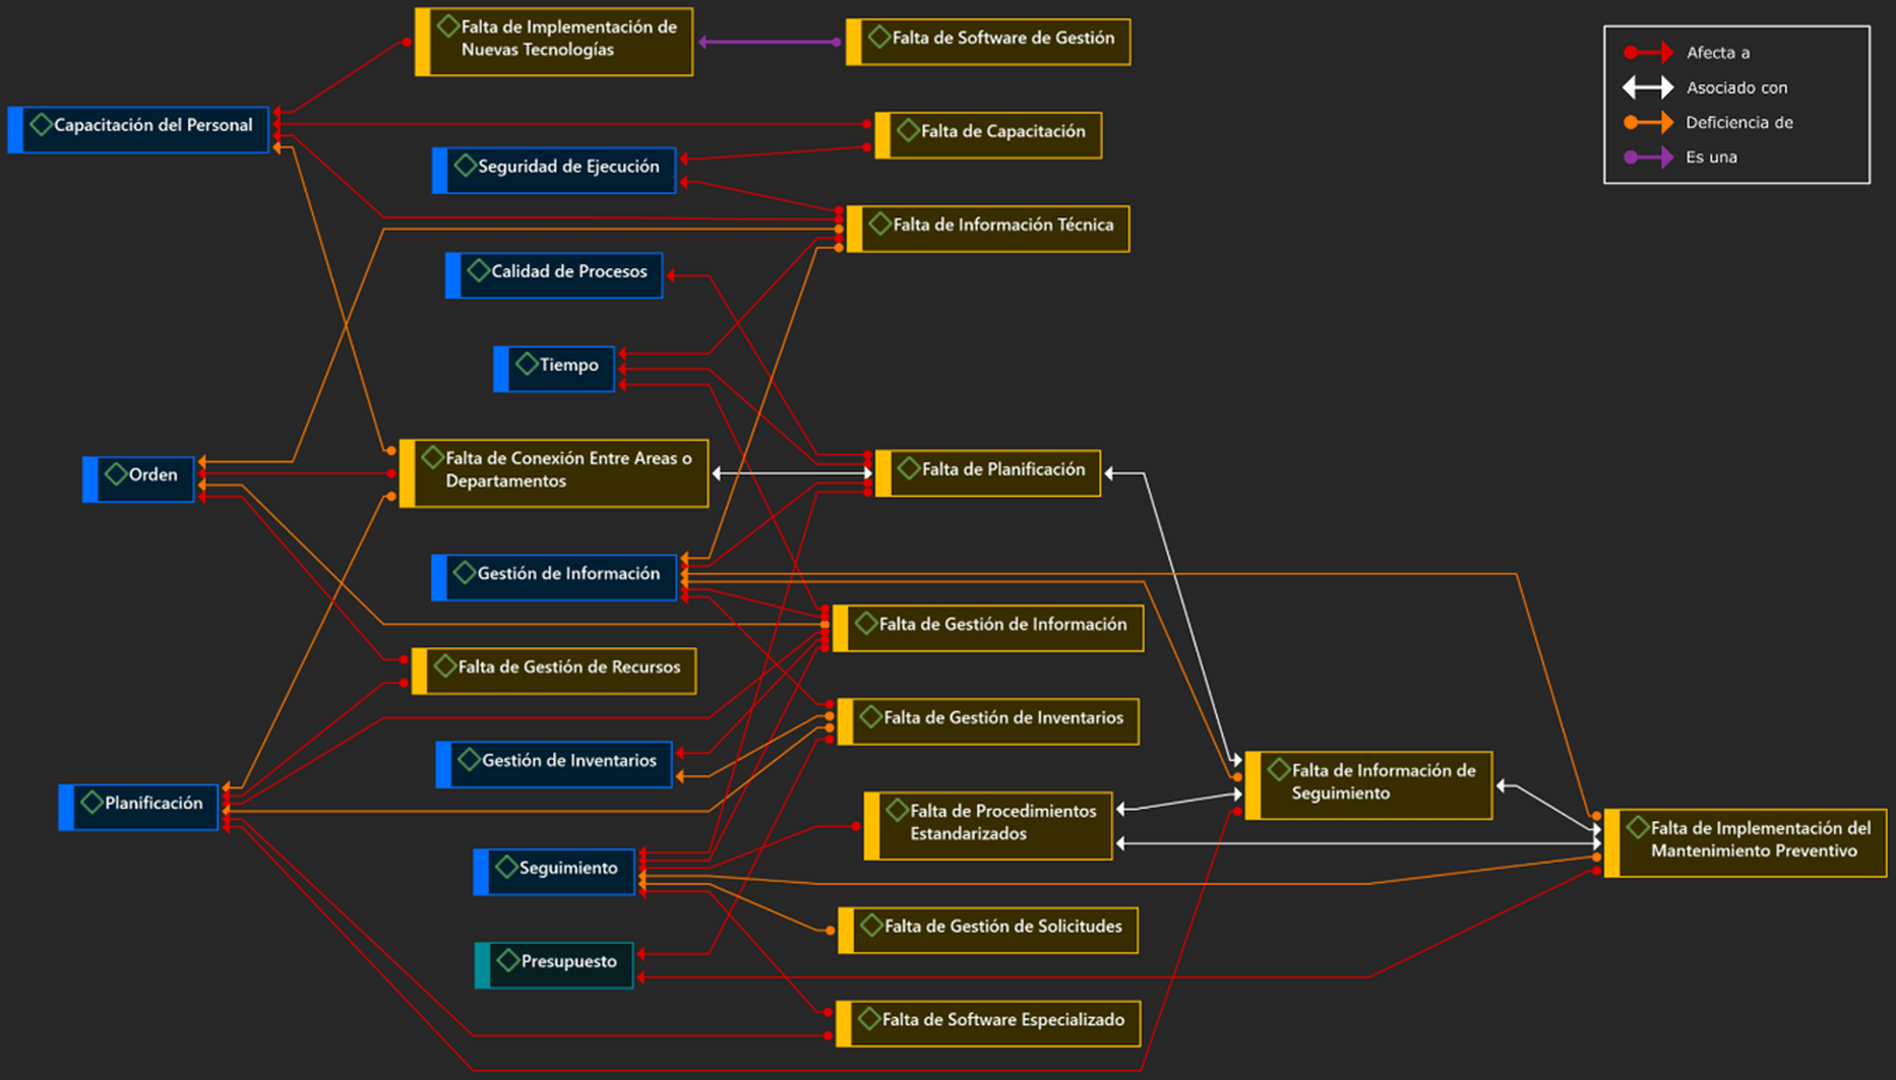
\includegraphics[width=\textwidth]{assets/figures/first_phase/network/img_semantic_network_problematic_situations.png}
    \label{fig:semantic_network_problematic_situations}
\end{figure}
\fixvspace{1}

        \subsubsection{Redes semánticas de los paneles}

            En base a la codificación de las encuestas, se elaboraron diagramas de redes semánticas que exponen la relación entre los paneles y las funcionalidades del aplicativo. Dichas redes, además, evidencian las conexiones entre las funcionalidades y la codificación de los distintos aspectos y conceptos de mantenimiento identificados en la red, especificando su tipo de relación para cada caso.
            
            \paragraph{Panel de cronograma de eventos}
            
                La red semántica mostrada en la Figura \ref{fig:semantic_network_schedule}, muestra un panel que tiene su implicación en la gestión y control de los tiempos de mantenimiento, siendo la planificación una propiedad del mismo. Los encuestados destacaron aspectos como la programación de fechas, así como notificación de las mismas. En cuanto a los conceptos de mantenimiento preventivo, la gestión de las intervenciones se asoció directamente con el concepto de la vida útil de los equipos.

                \begin{figure}[H]

    \caption{Relaciones semánticas del panel de cronograma}
    
    \centering
    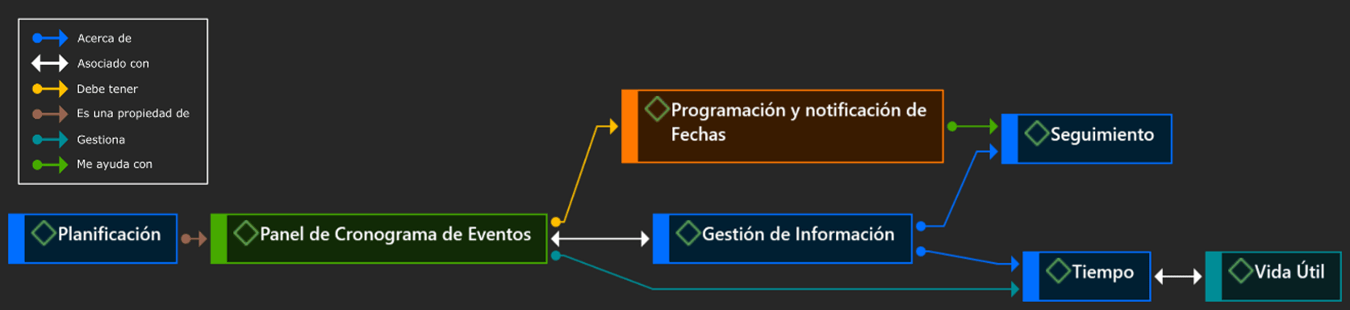
\includegraphics[width=1.0\textwidth]{assets/figures/first_phase/network/img_semantic_network_schedule.png}
    \label{fig:semantic_network_schedule}
    
\end{figure}
\vspace{-1.6\baselineskip}

            \paragraph{Panel de recursos multimedia}
            
                En la Figura \ref{fig:semantic_network_media_resources}, se presenta la red semántica para un panel que cubre el aspecto de gestión de información en cuanto a manuales, fichas técnicas y demás documentos asociados a los equipos y procesos de mantenimiento. Lo anterior es descrito como una ayuda para la capacitación del personal que realizará las diversas tareas de mantenimiento, al permitir al usuario, el acceso a información que favorece a la familiarización con los equipos así como a una mejora en la realización de los procedimientos.

                \begin{figure}[H]%htbp

    \caption{Relaciones semánticas del panel de recursos multimedia}
    
    \centering
    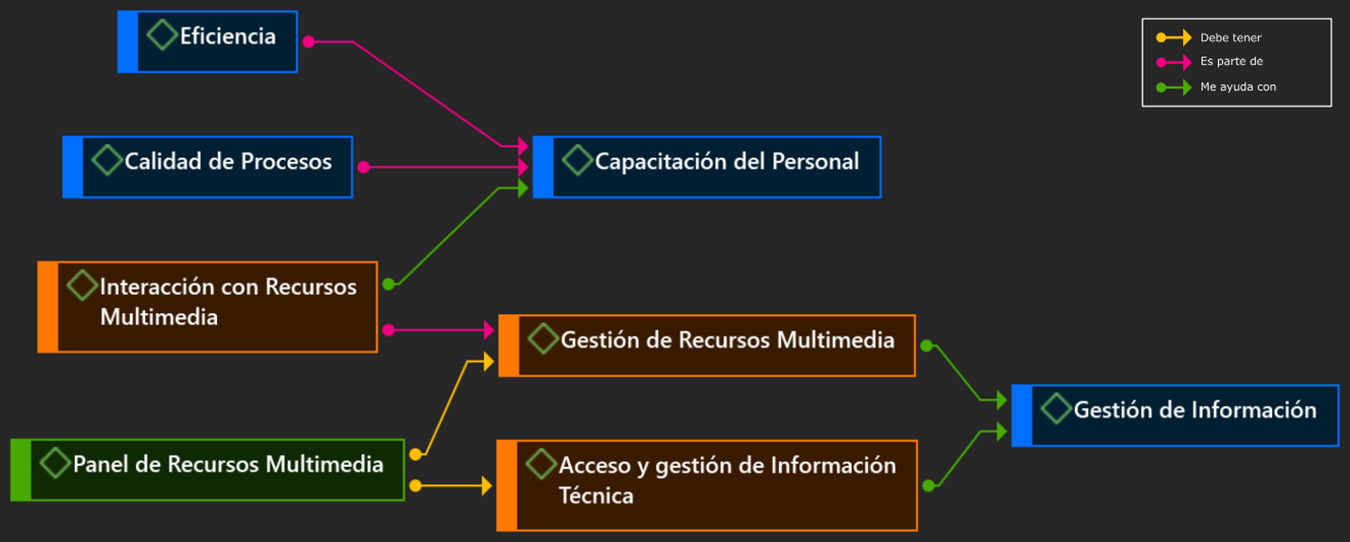
\includegraphics[width=1.0\textwidth]{assets/figures/first_phase/network/img_semantic_network_media_resources.png}
    \label{fig:semantic_network_media_resources}
    
\end{figure}
\vspace{-1.6\baselineskip}

            \paragraph{Panel de inventario}
            
                La red semántica presentada en la Figura \ref{fig:semantic_network_inventory} corresponde al Panel de Inventario, cuyo propósito principal es incorporar al aplicativo funcionalidades para la gestión de existencias de insumos antes y después de las intervenciones de mantenimiento, con el fin de facilitar el control de su disponibilidad y reducir posibles errores en su registro o conteo. De igual modo, se plantea la posibilidad de acceder a las características y especificaciones técnicas de los elementos registrados, permitiendo complementar la información necesaria para la planificación y ejecución de las actividades de mantenimiento. 

                \begin{figure}[H]

    \caption{Relaciones semánticas del panel de inventario}
    \centering
    
    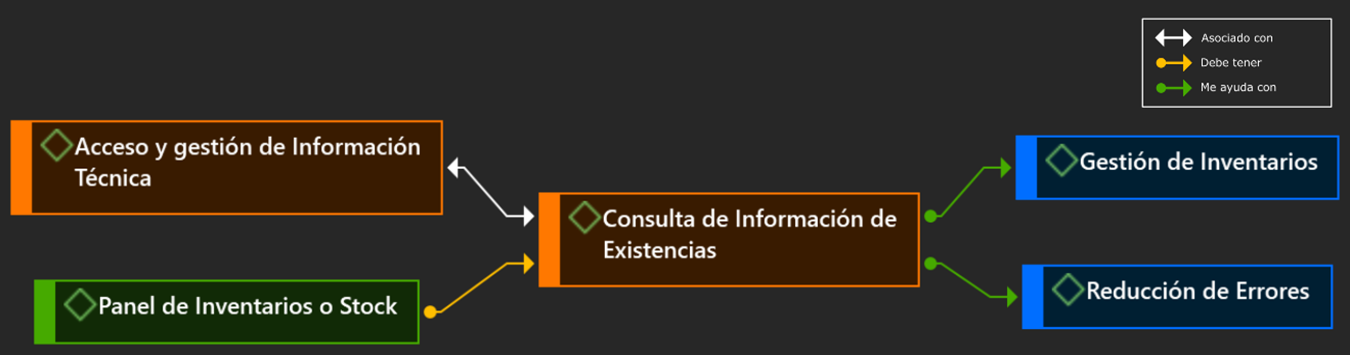
\includegraphics[width=1\textwidth]{assets/figures/first_phase/network/img_semantic_network_inventory.png}
    \label{fig:semantic_network_inventory}
    
\end{figure}
\fixvspace{1}

            \paragraph{Panel de realización de procedimientos}
            
                La red semántica de la Figura \ref{fig:semantic_network_procedures_development} evidencia relaciones entre diferentes elementos asociados al apoyo visual, acceso a información y asistencia durante la ejecución de tareas de mantenimiento preventivo. Entre las conexiones más destacadas se encuentran la interacción con objetos 3D, la presentación secuencial de procedimientos y la validación de tareas mediante listas de chequeo, características relacionadas con la comprensión de actividades y la reducción de errores durante la ejecución.

                Asimismo, conceptos como el acceso a información técnica y de seguimiento se vinculan con aspectos como la seguridad de ejecución, la eficiencia, el control de actividades y la calidad de los procesos. En conjunto, las relaciones identificadas sugieren que las herramientas basadas en realidad aumentada pueden funcionar no solo como apoyo visual, sino también como soporte integral para la gestión y ejecución del mantenimiento preventivo.

                \begin{figure}[H]%htbp

    \caption{Relaciones semánticas del panel de realización de procedimientos}
    
    \centering
    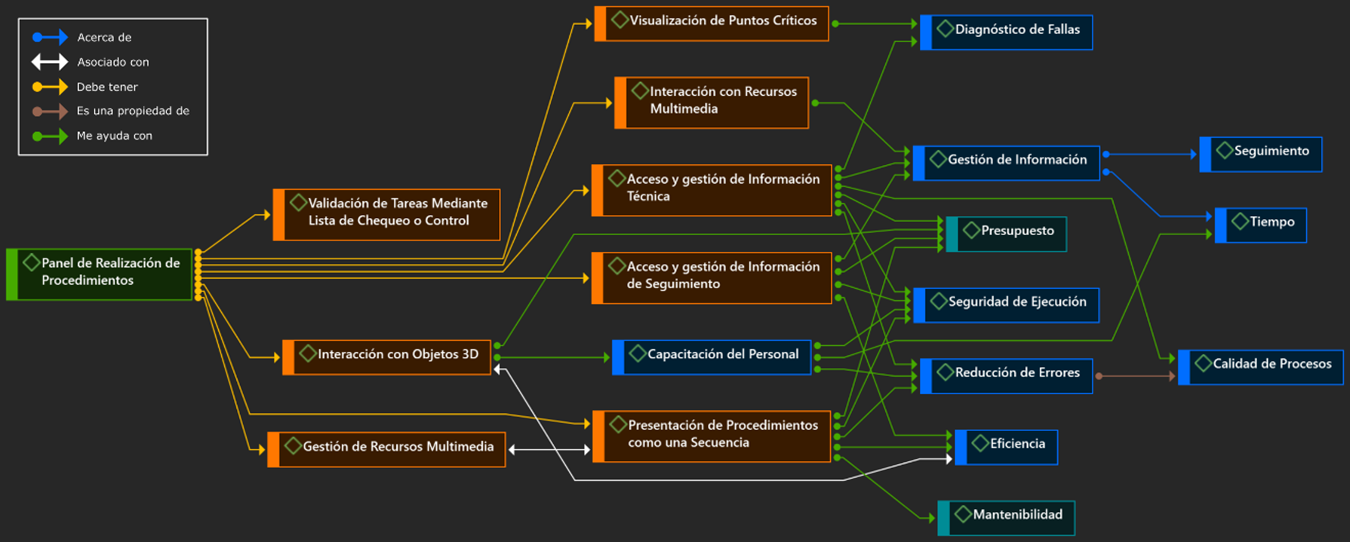
\includegraphics[width=1.0\textwidth]{assets/figures/first_phase/network/img_semantic_network_procedures_development.png}
    \label{fig:semantic_network_procedures_development}
    
\end{figure}
\vspace{-1.6\baselineskip}

            \paragraph{Panel de lista de procedimientos}
            
                Para este panel se obtuvo una red semántica que conecta cinco funcionalidades con aspectos de mantenimiento, tal y como se observa en la Figura \ref{fig:semantic_network_procedures_list}. Se destaca la presentación de una lista de instrucciones que organiza los procedimientos en una secuencia estructurada, lo cual coincide con el establecimiento de la estandarización para realizar las rutinas de mantenimiento de mayor calidad, que a su vez derive en  una disminución de los errores de ejecución. 

                \begin{figure}[H]
    \caption{Relaciones semánticas del panel de lista de procedimientos}
    \centering
    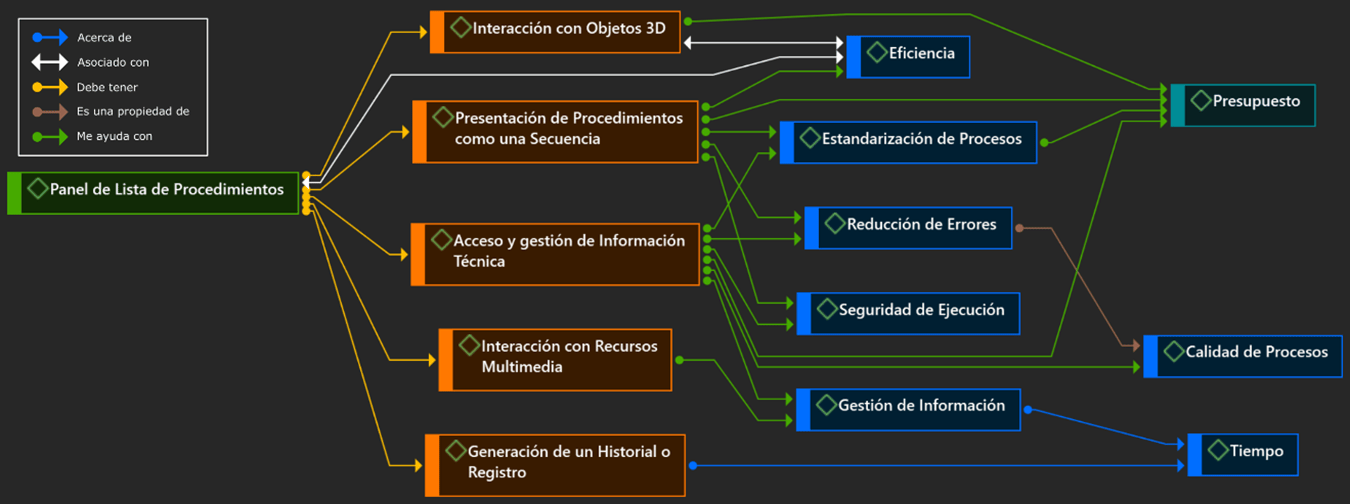
\includegraphics[width=\textwidth]{assets/figures/first_phase/network/img_semantic_network_procedures_list.png}
    \label{fig:semantic_network_procedures_list}
\end{figure}
\fixvspace{1}

            \paragraph{Panel de información técnica}
            
                El panel representado en esta red semántica (Figura \ref{fig:semantic_network_technical_information}) integra cinco funcionalidades, entre las cuales destaca el acceso y la gestión de distintos tipos de información bajo condiciones de conectividad limitada, ofreciendo una solución a una necesidad práctica identificada en los contextos de trabajo descritos por los entrevistados. Asimismo, se resalta la posibilidad de interactuar con diversos recursos multimedia dentro del aplicativo, los cuales facilitan la gestión de la información y se vinculan con los conceptos de seguimiento y tiempo, elementos esenciales para cualquier tipo de intervención.

                \begin{figure}[H]

    \caption{Relaciones semánticas del panel de información técnica}

    \centering
    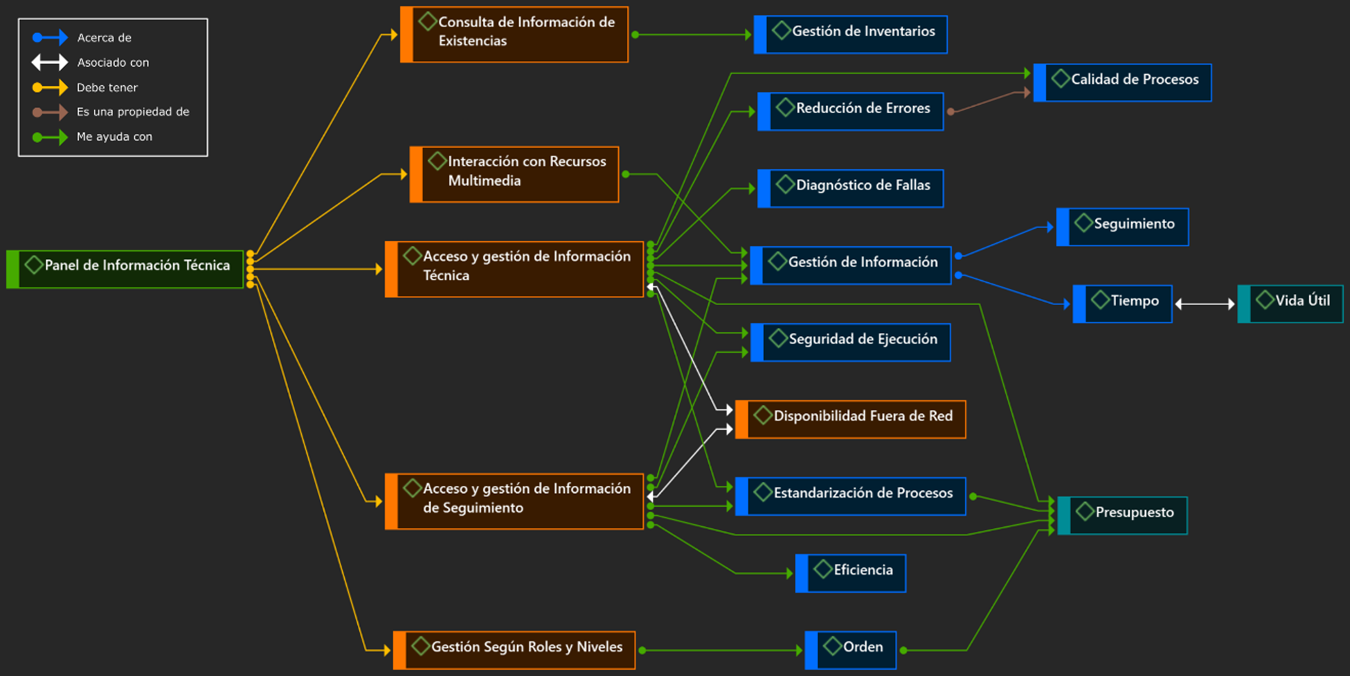
\includegraphics[width=1.0\textwidth]{assets/figures/first_phase/network/img_semantic_network_technical_information.png}
    \label{fig:semantic_network_technical_information}
    
\end{figure}
\vspace{-1.6\baselineskip}

    \subsection{Co-ocurrencia de datos}
        
        Uno de los elementos analizados, como complemento de las conexiones conceptuales representadas en las redes semánticas, fue la coocurrencia. Este concepto hace referencia a la aparición simultánea de dos o más códigos dentro de una porción de texto predefinida \parencite{ESCALANTE:2009}. A través de este análisis se buscó destacar la aparición de determinados códigos con mayor presencia, así como las relaciones establecidas entre ellos, resaltando aquellas coocurrencias que se presentaron con mayor frecuencia en las citas obtenidas de las encuestas. 

        \subsubsection{Diagramas Sankey}

            Para visualizar las relaciones más relevantes en cuanto a su coocurrencia, es decir en base a su densidad, se optó por el uso de diagramas Sankey. Estos diagramas ilustran por medio de caminos las relaciones entre entidades, permitiendo visualizar la proporción de un código o concepto en relación con otros \parencite{HECKER:SF}. A continuación se presentan los diagramas Sankey obtenidos:
            
            \paragraph{Diagrama de densidad de las funcionalidades}
            
                Las funcionalidades son aquellas prestaciones que se le dan al usuario y que van incluidas dentro de los distintos paneles o secciones gráficas del aplicativo. En la figura \ref{fig:sankey_functionalities} se muestran las funcionalidades identificadas en el proceso de categorización y la relevancia que los encuestados les dieron, basada en la cantidad de menciones. Las más destacadas fueron el acceso y gestión de la información técnica, acceso y gestión de información de seguimiento, interacción con objetos 3D y presentación de procedimientos como una secuencia. 

                \begin{figure}[H]

    \caption{Densidad de las funcionalidades del aplicativo resaltadas por los encuestados}
    
    \centering
    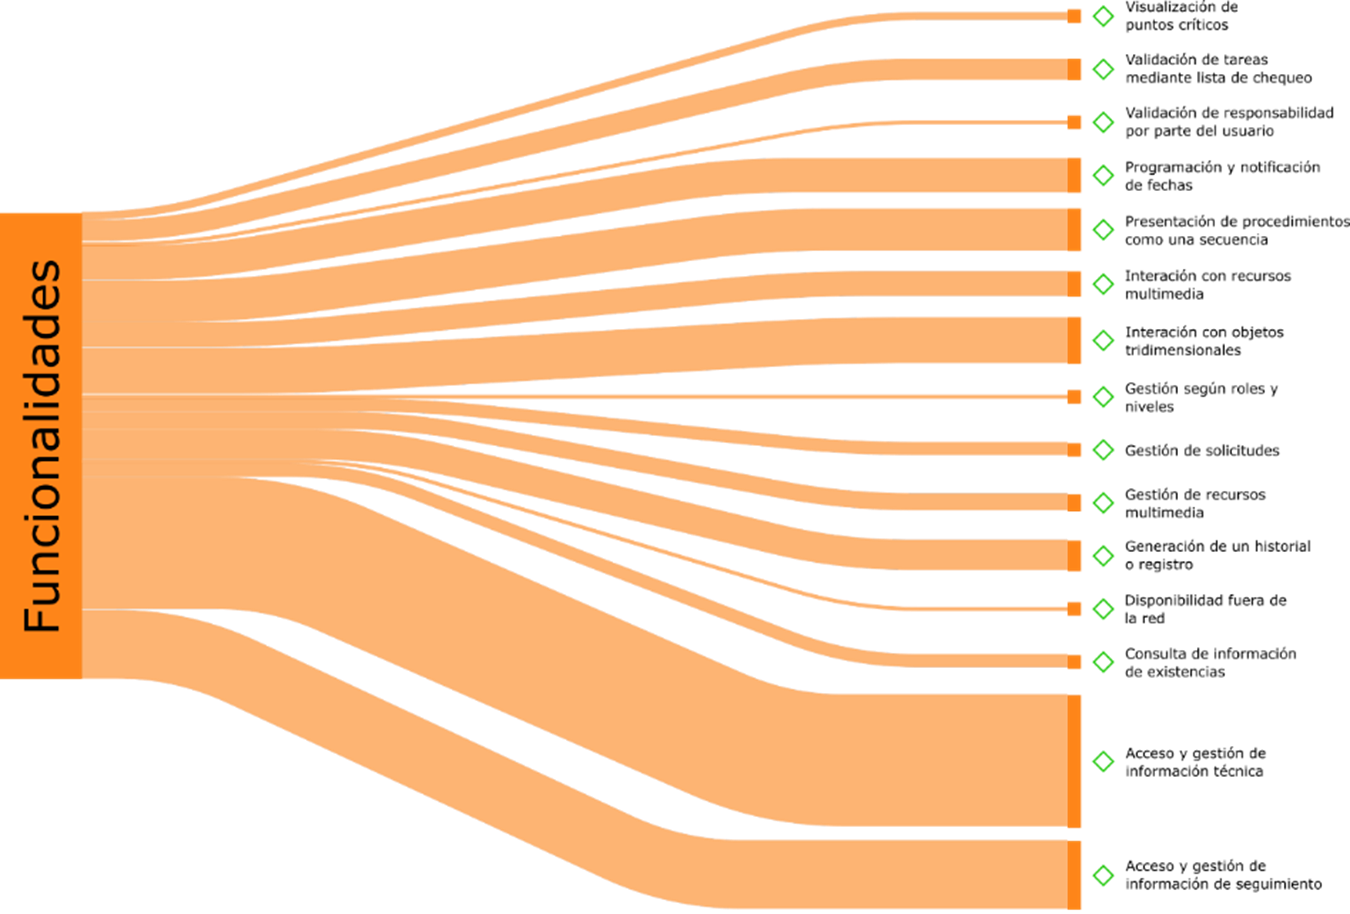
\includegraphics[width=0.8\textwidth]{assets/figures/first_phase/sankey/img_sankey_functionalities.png}
    \label{fig:sankey_functionalities}
    
\end{figure}
\vspace{-0.8\baselineskip}

            \paragraph{Diagrama de densidad de los paneles}
            
                En el diagrama de la Figura \ref{fig:sankey_panels} se identifican las propuestas de las secciones gráficas que pueden ser incorporadas en el aplicativo identificadas en las citas, donde se observa una alta mención al panel de información técnica prevaleciendo la importancia de los aspectos de gestión de información técnica específica de los ítems mantenibles y del mismo modo se observa una gran densidad al panel de realización de procedimientos y el de lista de procedimientos, siendo estos una guía en el desarrollo de las distintas intervenciones de mantenimiento con el uso de realidad aumentada.

                \begin{figure}[H]
    \caption{Densidad de los paneles del aplicativo de mantenimiento}
    \centering
    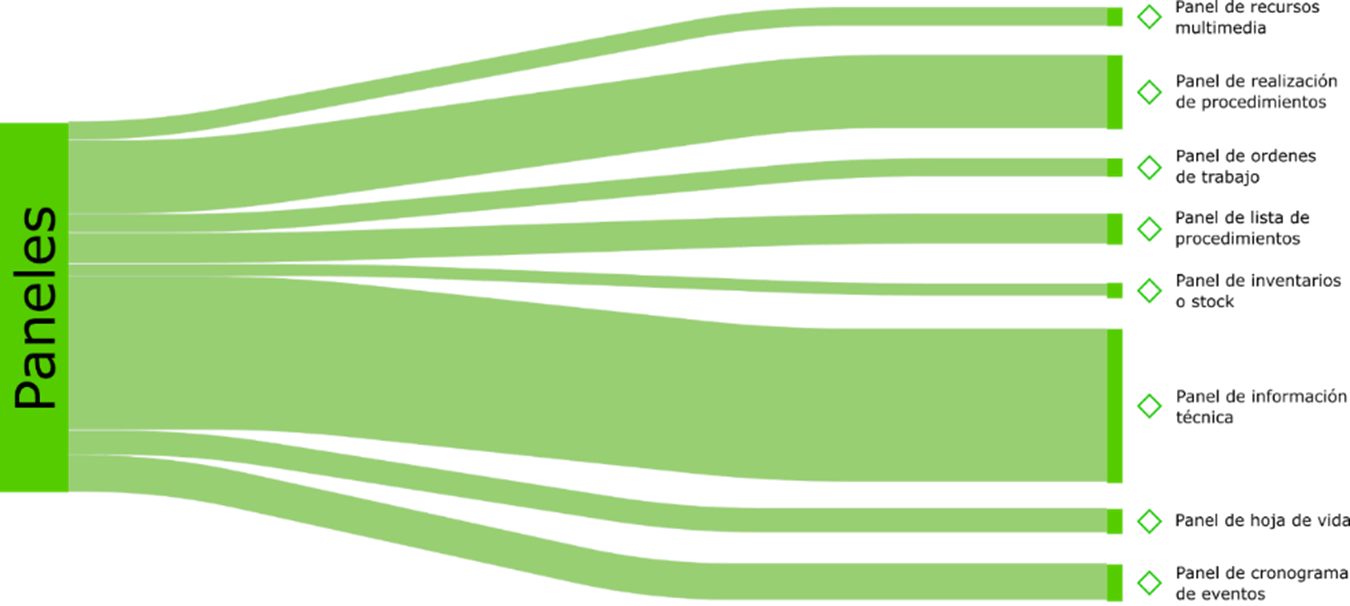
\includegraphics[width=0.8\textwidth]{assets/figures/first_phase/sankey/img_sankey_panels.png}
    \label{fig:sankey_panels}
\end{figure}
\fixvspace{0}
            
            \paragraph{Diagrama de co-ocurrencia entre aspectos y funcionalidades de mantenimiento}
            
                Este diagrama, ilustrado en la Figura \ref{fig:sankey_coocurrence_functionalities_aspecs}, muestra la relación entre las funcionalidades (representadas en naranja) y los distintos aspectos del mantenimiento (en azul). Donde se observa un patrón de convergencia que reune múltiples aspectos de mantenimiento en una misma funcionalidad, lo cual podría indicar que dicha funcionalidad es un elemento central para el diseño y la experiencia de los usuarios, al ser considerado desde diferentes puntos.
            
                \begin{figure}[H]

    \caption{Co-ocurrencia entre funcionalidades y aspectos de mantenimiento}
    
    \centering
    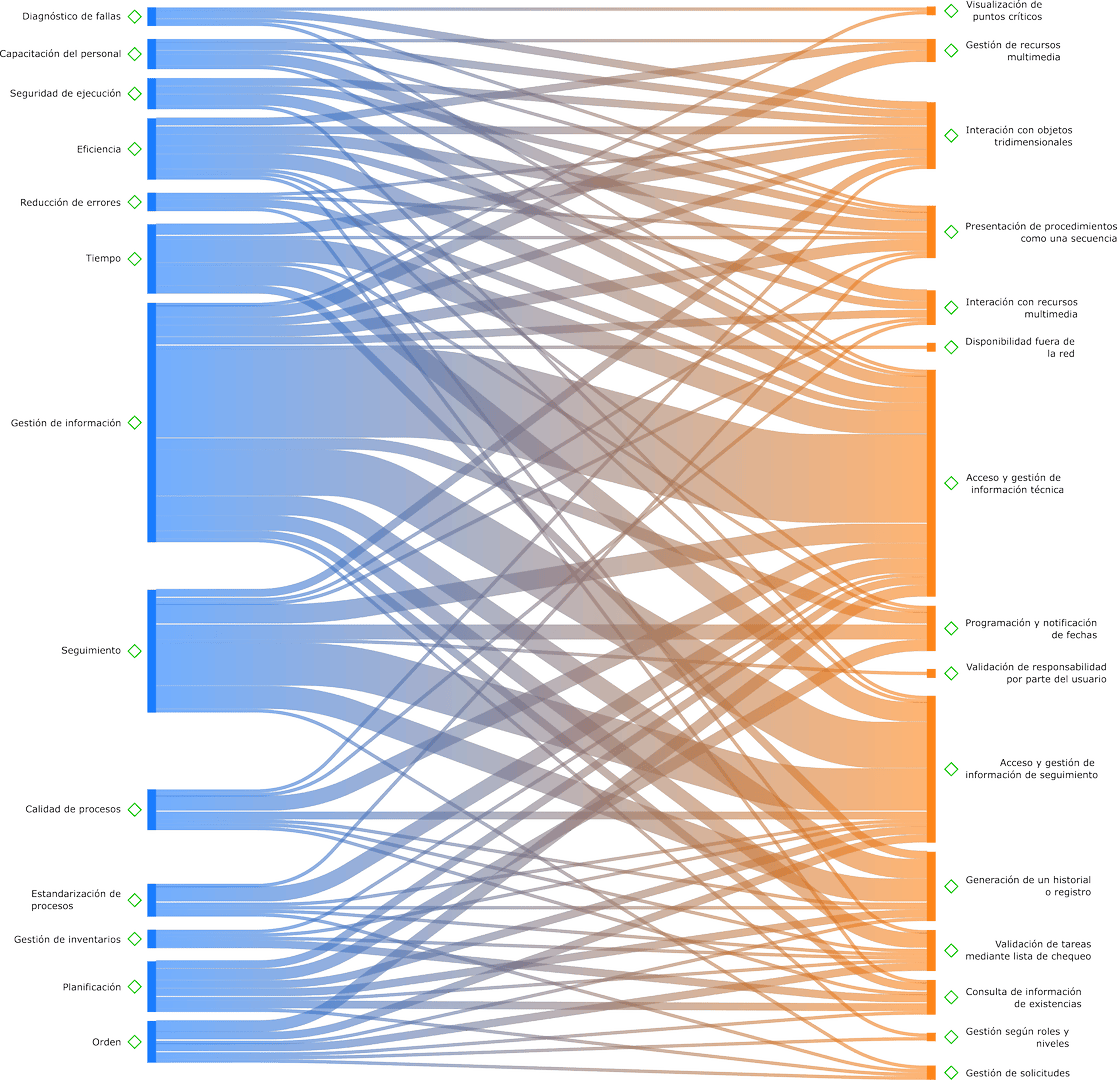
\includegraphics[width=1.0\textwidth]{assets/figures/first_phase/sankey/img_sankey_coocurrence_functionalities_aspecs.png}
    \label{fig:sankey_coocurrence_functionalities_aspecs}
    
\end{figure}
\vspace{-1.6\baselineskip}

            \paragraph{Diagrama de co-ocurrencia entre paneles y funcionalidades}
            
                El diagrama de Sankey de la Figura \ref{fig:sankey_coocurrence_panels_functionalities} muestra las conexiones entre los paneles propuestos en las encuestas (representados en verde) y las funcionalidades (en naranja). En dicho diagrama, se observa un patrón de divergencia en el que los paneles de mayor densidad se vinculan con múltiples funcionalidades, lo cual podría indicar que estas son secciones relevantes para ser incorporadas en el desarrollo de la aplicación de realidad aumentada.

                \begin{figure}[H]
    \caption{Co-ocurrencia entre los paneles propuestos y funcionalidades de mantenimiento}
    \centering
    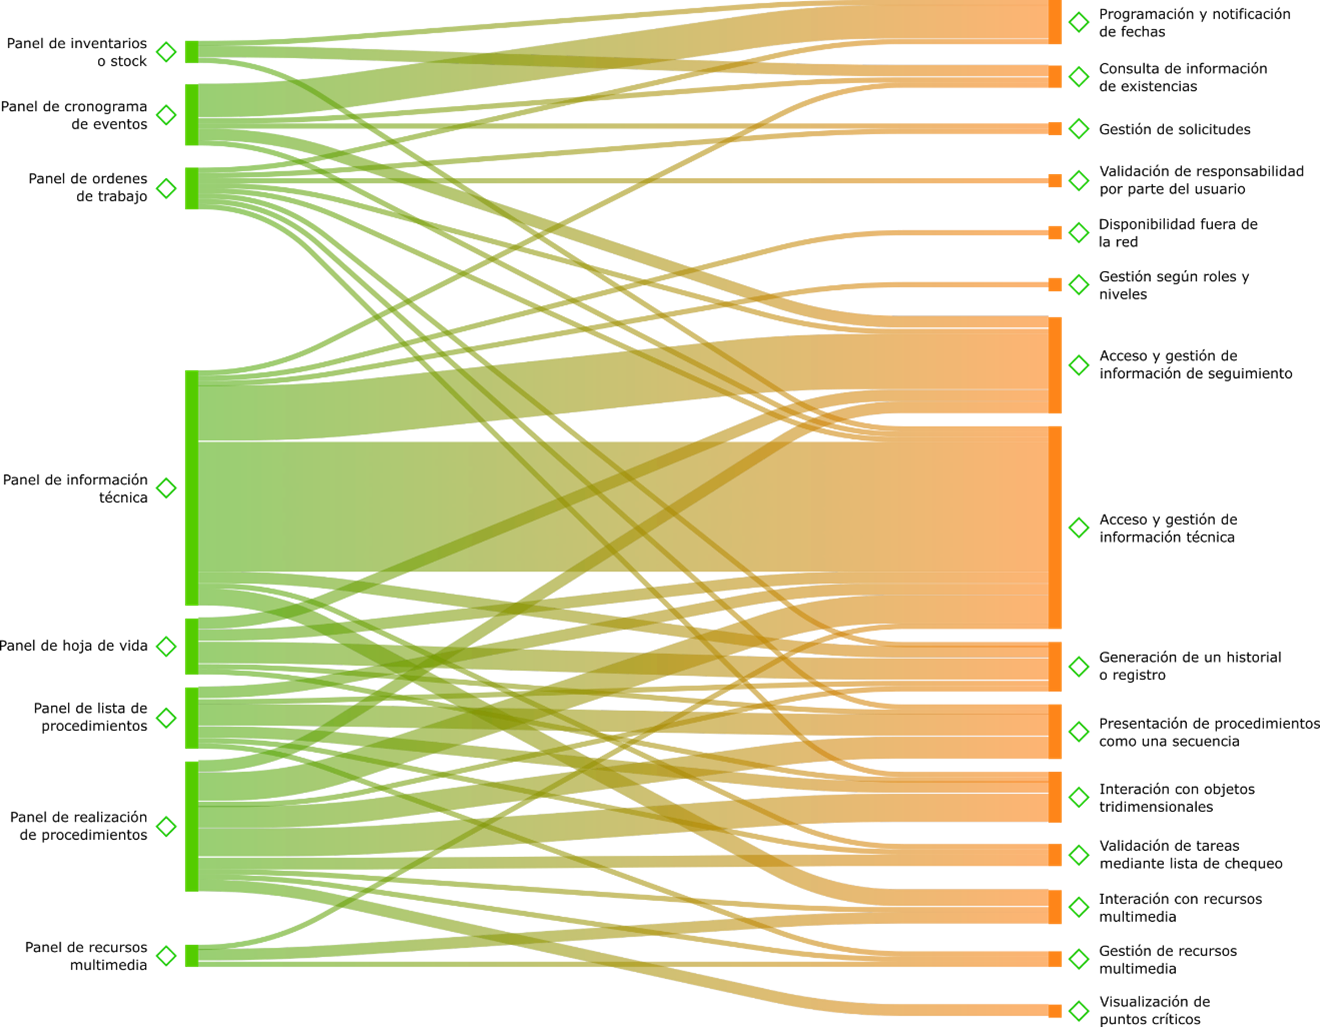
\includegraphics[width=\textwidth]{assets/figures/first_phase/sankey/img_sankey_coocurrence_panels_functionalities.png}
    \label{fig:sankey_coocurrence_panels_functionalities}
\end{figure}
\fixvspace{1}

    \subsection{Requerimientos de la aplicación}

        A partir del análisis cualitativo de las encuestas, y como conclusión de la primera fase de desarrollo, se establecieron los paneles que conformarán la interfaz de la aplicación de realidad aumentada.

        \subsubsection{Panel para la gestión de la información técnica de los equipos}

            Este panel permite almacenar y gestionar la información técnica correspondiente a los equipos o ítems sujetos a mantenimiento. Con el propósito de facilitar la identificación precisa de cada equipo dentro de la aplicación, y de acuerdo con los fundamentos teóricos establecidos, se registrarán los siguientes datos:

            \begin{itemize}
                \item Código del equipo.
                \item Nombre.
                \item Tipo de máquina.
                \item Ubicación.
                \item Marca.
                \item Modelo.
                \item Número de serie.
                \item Año de fabricación.
                \item Precio inicial.
                \item Fecha de adquisición.
                \item Observaciones generales.
                \item Datos del motor.
                \item Imagen identificativa.
            \end{itemize}

        \subsubsection{Panel para la ejecución de procedimientos}

            Esta sección opera como una guía para la realización asistida de las diversas actividades de mantenimiento mediante el uso de realidad aumentada. Su diseño se fundamenta en el análisis de coocurrencia derivado de las encuestas, a partir del cual se definieron las siguientes funcionalidades principales:

            \begin{itemize}
                \item Gestión de archivos multimedia, tales como imágenes y modelos 3D.
                \item Interacción con recursos multimedia dentro de un entorno de realidad aumentada.
                \item Presentación de procedimientos en un formato secuencial, estructurado por pasos y operaciones.
            \end{itemize}

        \subsubsection{Panel de escáner de códigos QR}

            Este panel proporciona al usuario una interfaz basada en la cámara del dispositivo móvil, habilitada para la detección de marcadores y la posterior redirección en el sistema. Su objetivo es permitir el escaneo de los códigos QR para agilizar el acceso a los detalles y a las actividades de mantenimiento en realidad aumentada de cada máquina. Dada su importancia en el flujo de interacción, se ha establecido como la pantalla principal de la aplicación.

        \subsubsection{Panel de cronograma de eventos}

            En este panel, el usuario tiene la capacidad de registrar anotaciones relacionadas con las fechas de las intervenciones de mantenimiento, facilitando el control y cumplimiento de su periodicidad. Adicionalmente, se integra un sistema de notificaciones para alertar sobre la proximidad de las tareas programadas, contribuyendo a una mejor organización del tiempo. Con base en la revisión teórica, los datos principales a registrar y presentar son:

            \begin{itemize}
                \item Nombre del evento de mantenimiento.
                \item Descripción de la actividad.
                \item Categoría del mantenimiento.
                \item Fechas de intervención.
                \item Intervalos o recurrencia de la actividad.
            \end{itemize}

    \subsection{Restricciones de la aplicación}

        Con base en el alcance de los objetivos y los resultados de las encuestas, se establecieron las siguientes limitaciones técnicas para el desarrollo de la aplicación de realidad aumentada:

        \begin{enumerate}

            \item \textbf{Independencia de red:} La arquitectura del sistema opera bajo un enfoque fuera de línea (offline), por lo que las funcionalidades están restringidas a la ejecución local en el dispositivo para garantizar su operación en entornos de baja o nula conectividad a internet.
            
            \item \textbf{Reconocimiento espacial:} El despliegue de los elementos de realidad aumentada depende exclusivamente del seguimiento de marcadores físicos (rastreo de imágenes), prescindiendo de la integración y entrenamiento de modelos de aprendizaje automático.
            
            \item \textbf{Compatibilidad tridimensional:} El motor de renderizado restringe la importación y visualización de modelos 3D de forma exclusiva al estándar glTF, limitándose estrictamente a su codificación o formato binario (.glb).
            
            \item \textbf{Soporte multimedia:} La carga y visualización de recursos en dos dimensiones admite únicamente formatos de imagen estática, excluyendo el procesamiento de medios continuos o audiovisuales.
            
        \end{enumerate}